%!TEX root=../document.tex

\section{Ergebnisse}
\label{sec:Ergebnisse}
\subsection{XNOR}
Zuerst musste wieder die Topologie angepasst werden:

\begin{lstlisting}[language=c]
	topologie{ 2,4,1 }
\end{lstlisting}

Das Trainingsset wurde wie in der Aufgabenbeschreibung definiert, und dieses wurde insgesamt \textbf{10.000} mal dem NN antrainiert. 

Nachdem die Ausgabe wieder nur einem Output Node angepasst wurde, konnte man folgendes Ergebnis erkennen:

\begin{minipage}{\linewidth}
	\centering
	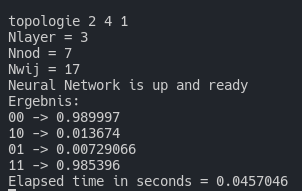
\includegraphics[width=0.6\linewidth]{images/1}
\end{minipage}

\subsection{NAND}
Es wurde die Topologie von XNOR übernommen und es wurde lediglich das Trainingsset angepasst um die Funktionsweise eines NAND nachzubauen. Somit ist folgende Ausgabe zustande gekommen:

\begin{minipage}{\linewidth}
	\centering
	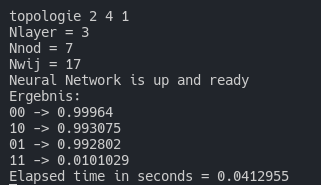
\includegraphics[width=0.6\linewidth]{images/2}
\end{minipage}

\subsection{XNOR \& NAND}
Erstmals wurde, daher nun \textbf{2} Outputs zu erwarten sind, wieder die Topologie angepasst:

\begin{lstlisting}[language=c]
	topologie{ 2,5,2 }
\end{lstlisting}

Im Trainingsset wurden nun ein weiter Output Node hinzugefügt welcher bei jedem Element gesetzt wurde. Nach dem Trainieren hat sich folgendes Ergebnis ergeben:

\begin{minipage}{\linewidth}
	\centering
	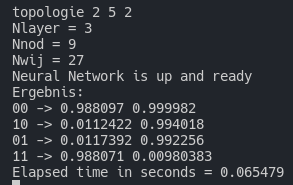
\includegraphics[width=0.6\linewidth]{images/3}
\end{minipage}

